\chapter{Finite element method: formulation}

\disclaimer

\section{Introduction}
The objective of this section is threefold.  We first introduce finite elements for reference triangles. We then discuss the assembly of finite elements to construct a finite element space.  We finally discuss approximation properties of these finite element spaces.


\section{Triangulation}
We first introduce a \emph{triangulation} of $\Omega \subset \RR^d$.  A triangulation
\begin{equation*}
  \calT_h \equiv \{ K_i \}_{i=1}^{n_e}
\end{equation*}
is a set of non-overlapping elements $K_1, \dots, K_{n_e}$ such that union of the closure of the elements cover the domain: $\cup_{i=1}^{n_e} \overline K_i = \overline \Omega$.   (We consider the closure of the elements because we consider each element to be open.) An example of triangulation of a square domain $\Omega$ is shown in Figure~\ref{fig:fe_mesh_p1}. The triangulation comprise $n_e = 9$ triangular elements, which are delineated by $n_v = 9$ vertices.  The subscript $h$ of the triangulation $\calT_h$ signifies the maximum diameter of the elements in the triangulation; specifically, $h \equiv \max_{i} \text{diam}(K_i)$, where $\text{diam}(K_i)$ is the diameter of the smallest ball that inscribes the element $K_i$.  Intuitively (and as we will see more formally), the finite element spaces associated with a sequence of triangulations get richer as $h$ decreases.  In general, a triangulation comprises line segments in one dimension, triangles or quadrilaterals in two dimension, and tetrahedrons or hexahedrons in three dimensions.


\begin{figure}
  \centering
  \subfigure[mesh]{
    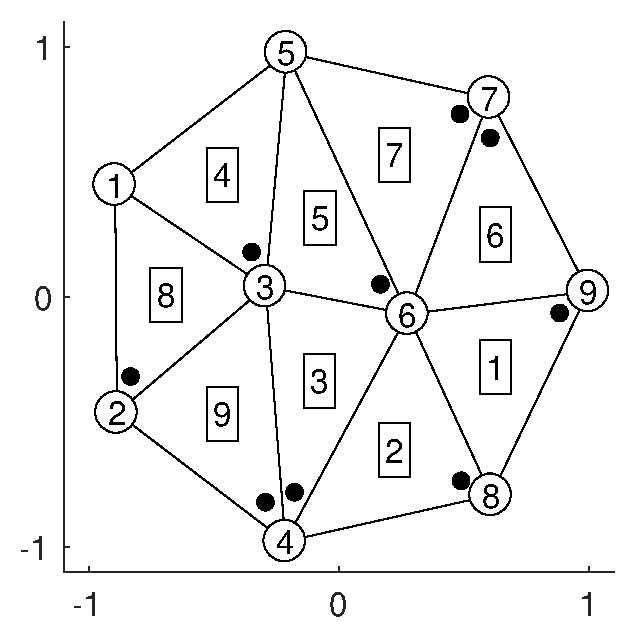
\includegraphics[width=0.4\textwidth]{fe_mesh_p1}
  }
  \caption{Triangulation.}
  \label{fig:fe_mesh_p1}
\end{figure}

While mathematically a triangulation is simply a collection of non-overlapping elements, we need a convenient means to represent the triangulation on a computer.  One approach is to store tables of \emph{node coordinates} and \emph{element-node connectivities}.  Tables~\ref{tb:fe_mesh_p1_coord} and \ref{tb:fe_mesh_p1_tri} are respectively the coordinate and connectivity tables associated with the triangulation shown in Figure~\ref{fig:fe_mesh_p1}. The connectivity table indicates that, for instance, element 5 is delineated by the nodes 6, 5, and 3; the coordinate table then indicates that the coordinates of these three nodes are $(0.28,-0.07)$, $(-0.21,0.98)$, and $(-0.29,0.04)$, respectively.  Note that, in Figure~\ref{fig:fe_mesh_p1}, for each triangle, we indicate the first of the three nodes that delineate the triangle by a dot ($\bullet$); with this convention we have identical information presented in Figure~\ref{fig:fe_mesh_p1} in a visual form and Tables~\ref{tb:fe_mesh_p1_coord} and \ref{tb:fe_mesh_p1_tri} in an array form.

\begin{table}
  \centering
  \caption{Node coordinate and connectivity table for mesh shown in Figure~\ref{fig:fe_mesh_p1}.  \label{tb:fe_mesh_p1}}
    \subfigure[coordinates]{
      \label{tb:fe_mesh_p1_coord}
    \begin{tabular}{c|cc}
      node & $x_1$ & $x_2$ \\
      \hline
      $1$ & $-0.89$ & $\hphantom{-}0.45$ \\ 
      $2$ & $-0.89$ & $-0.46$ \\ 
      $3$ & $-0.29$ & $\hphantom{-}0.04$ \\ 
      $4$ & $-0.21$ & $-0.98$ \\ 
      $5$ & $-0.21$ & $\hphantom{-}0.98$ \\ 
      $6$ & $\hphantom{-}0.28$ & $-0.07$ \\ 
      $7$ & $\hphantom{-}0.60$ & $\hphantom{-}0.80$ \\ 
      $8$ & $\hphantom{-}0.61$ & $-0.79$ \\ 
      $9$ & $\hphantom{-}1.00$ & $\hphantom{-}0.02$ \\ 
    \end{tabular}
  }
    \subfigure[connectivity]{
          \label{tb:fe_mesh_p1_tri}
    \begin{tabular}{c|ccc}
      element & node 1 & node 2 & node 3 \\
      \hline
      $1$ & $9$ & $6$ & $8$ \\ 
      $2$ & $8$ & $6$ & $4$ \\ 
      $3$ & $4$ & $6$ & $3$ \\ 
      $4$ & $3$ & $5$ & $1$ \\ 
      $5$ & $6$ & $5$ & $3$ \\ 
      $6$ & $7$ & $6$ & $9$ \\ 
      $7$ & $7$ & $5$ & $6$ \\ 
      $8$ & $2$ & $3$ & $1$ \\ 
      $9$ & $4$ & $3$ & $2$ \\ 
    \end{tabular}
    }
\end{table}

The task of generating a triangulation for a given domain is called \emph{mesh generation} and a program that carries out the task is called a \emph{mesh generator} or \emph{mesher}.  Mesh generation is a non-trivial task.  In fact, the development of algorithms that can robustly and automatically generate high-quality triangulation for complex geometries in three dimensions is an area of ongoing research.  Nevertheless, because mesh generation is essential for any finite element discretization, there are many commercial and open-source meshers.  Here we name a few user-friendly, open-source meshers:
\begin{itemize}
\item \texttt{triangle}. A robust two-dimensional mesher written in C that generates meshes with a guaranteed quality certificate in terms of the minimal angle.
\item \texttt{tetgen}. A popular three-dimensional mesher written in C.
\item \texttt{distmesh}.  A user-friendly mesher written in \textsc{Matlab} for implicit domain geometries represented by level sets. 
\end{itemize}
The mesh shown in Figure~\ref{fig:fe_mesh_p1} was in fact generated by \texttt{distmesh}.  We will extensively use \texttt{distmesh} to generate meshes in this course as it is implemented in \textsc{Matlab} and is easy to use.


\section{Approximation spaces}
We now introduce \emph{approximation spaces} for $\calV$.  An approximation space is a finite-dimensional subspace space of $\calV$ with which we can approximate functions in $\calV$.  For concreteness, we consider a piecewise-polynomial approximation space associated with the triangulation $\calT_h$. For simplicity, we first consider the case $\calV \equiv H^1(\Omega)$:
\begin{equation*}
  \calV_h \equiv \{ v \in \calV \equiv H^1(\Omega) \ | \ v|_K \in \PP^p(K), \ K \in \calT_h \},
  \label{eq:fe_Vh}
\end{equation*}
where $\PP^p(K)$ is the space of polynomials of degree at most $p$ over $K$.
We note the two requirements: $v \in \calV_h$ must belong to $\calV \equiv H^1(\Omega)$; 
%We note the two requirements: $v \in \calV_h$ must belong to $\calV \subset H^1(\Omega)$ and in particular satisfy the essential boundary conditions;
$v$ restricted to any element $K \in \calT_h$, $v|_K$, must be a polynomial of degree $p$. Figure~\ref{fig:fe_fun_p1} shows an example of a function in a linear ($\PP^1$) finite element space,
\begin{equation}
  \calV_h \equiv \{ v \in \calV \equiv H^1(\Omega) \ | \ v|_K \in \PP^1(K), \ K \in \calT_h \},
  \label{eq:fe_lin_Vh}
\end{equation}
associated with the mesh shown in Figure~\ref{fig:fe_mesh_p1}.

\begin{figure}
  \centering
  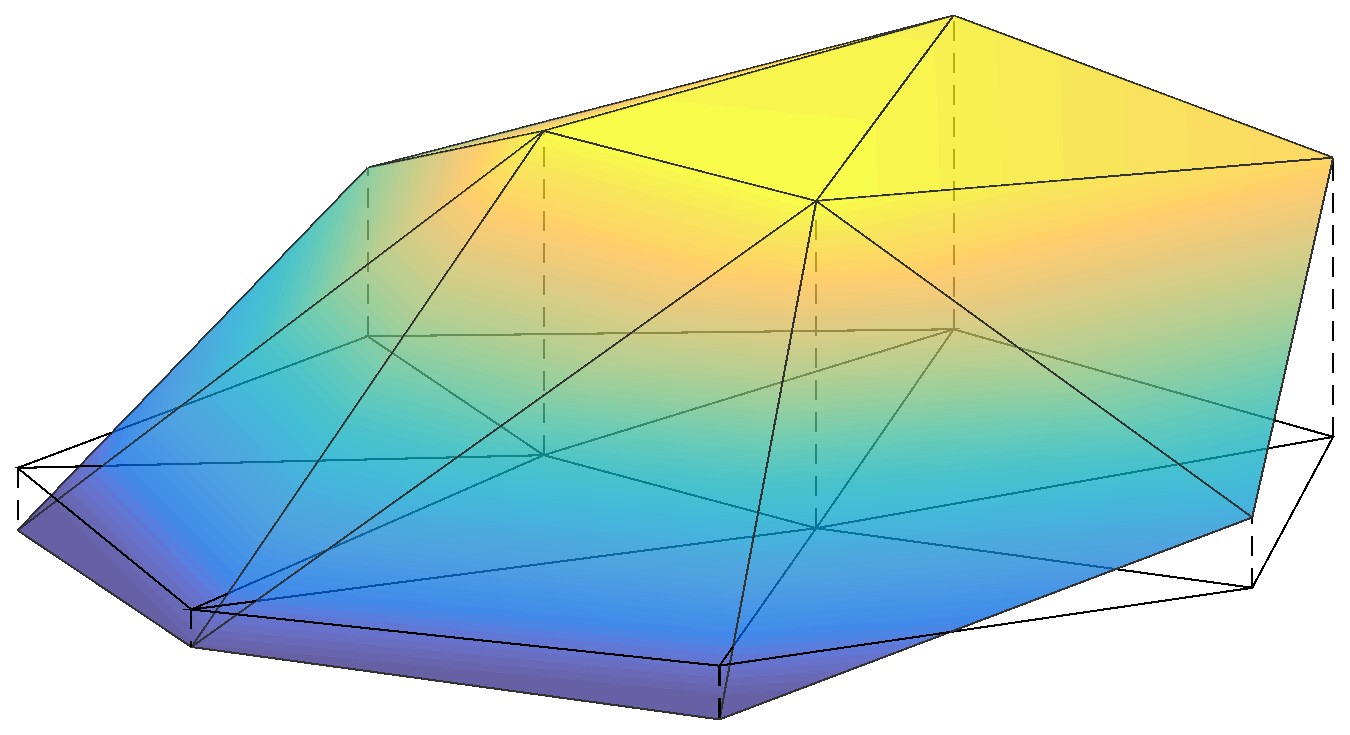
\includegraphics[width=0.45\textwidth]{fe_fun_p1}
  \caption{A function in a linear finite element space.}
  \label{fig:fe_fun_p1}
\end{figure}

We note that the condition $\calV_h \subset \calV \subset H^1(\Omega)$ means that the weak derivative of functions must be square integrable (in the Lebesgue sense); for piecewise polynomials, the condition is satisfied if and only if the function is continuous.  To see this, we observe the following.  If a function is continuous and piecewise polynomial, the weak first derivative is potentially discontinuous but is piecewise polynomial and hence is square integrable; the function hence is in $H^1(\Omega)$.  If a function is not continuous across element interfaces, then the weak first derivative generates delta distributions at the interfaces and hence is not in $L^2(\Omega)$; recall for instance a concrete example for a Heaviside-like function in Section~\ref{sec:posnd_sobolev}. Hence, for a piecewise polynomial function, the continuity is the necessary and sufficient condition for the function to be in $H^1(\Omega)$. 

We now need a convenient means to describe functions in $\calV_h$ given by~\eqref{eq:fe_lin_Vh}, such as the one shown in Figure~\ref{fig:fe_fun_p1}.  Specifically, we need to pick \emph{global degrees of freedom} with which we can uniquely describe any function in $\calV_h$. To this end, we introduce a \emph{basis} for the linear space $\calV_h$.  We recall that a set of functions $\{ \phi_i \}_{i=1}^n$ is a basis for $\calV_h$ if the set (i) spans $\calV_h$ and (ii) is linearly independent. The first requirement implies that any $w \in \calV_h$ can be expressed as a linear combination of $\{ \phi_i \}_{i=1}^n$.  The second requirement implies that the coefficients associated with the representation of $w \in \calV_h$ in terms of $\{ \phi_i \}_{i=1}^n$ is unique.  In other words, if $\{ \phi_i \}_{i=1}^n$ is a basis for $\calV_h$, then for any $w \in \calV_h$ there exists a unique $\hat w \in \RR^n$ such that
\begin{equation*}
  w = \sum_{j=1}^n \hat w_j \phi_j
\end{equation*}
for $n = \text{dim}(\calV_h)$.

While the choice of a basis is not unique, one convenient choice is a \emph{Lagrange basis} or \emph{nodal basis}.  Nodal basis comprises functions that take on the value of 1 at the associated node and 0 at all other nodes:
\begin{equation}
  \phi_j(x_i) = \delta_{ij},
  \label{eq:fe_lagrange_basis_prop}
\end{equation}
where $\delta_{ij}$ is the Kronecker delta so that $\delta_{ij} = 1$ if $i = j$ and $\delta_{ij} = 0$ if $i \neq j$. Figure~\ref{fig:fe_shape_global_p1} shows an example of a basis function, $\phi_3$, for the linear finite element space~\eqref{eq:fe_lin_Vh} associated with the mesh shown in Figure~\ref{fig:fe_mesh_p1}.  For $\calV_h$ defined by~\eqref{eq:fe_lin_Vh}, there are nine nodal basis functions, one associated with each node.  We also observe that the set of the nine functions indeed forms a basis: the set is linearly independent and spans the space. The set is linearly independent because $\sum_{j=1}^n \hat w_j \phi_j = 0$ implies $\sum_{j=1}^n \hat w_j \phi_j(x_i) = 0$, $\forall i =1,\dots,n$, which in turn implies $\hat w_j = 0$, $j = 1,\dots,n$.  The set spans the space because the piecewise linear polynomial space is nine dimensional and the linearly independent set contains nine functions.

\begin{figure}
  \centering
  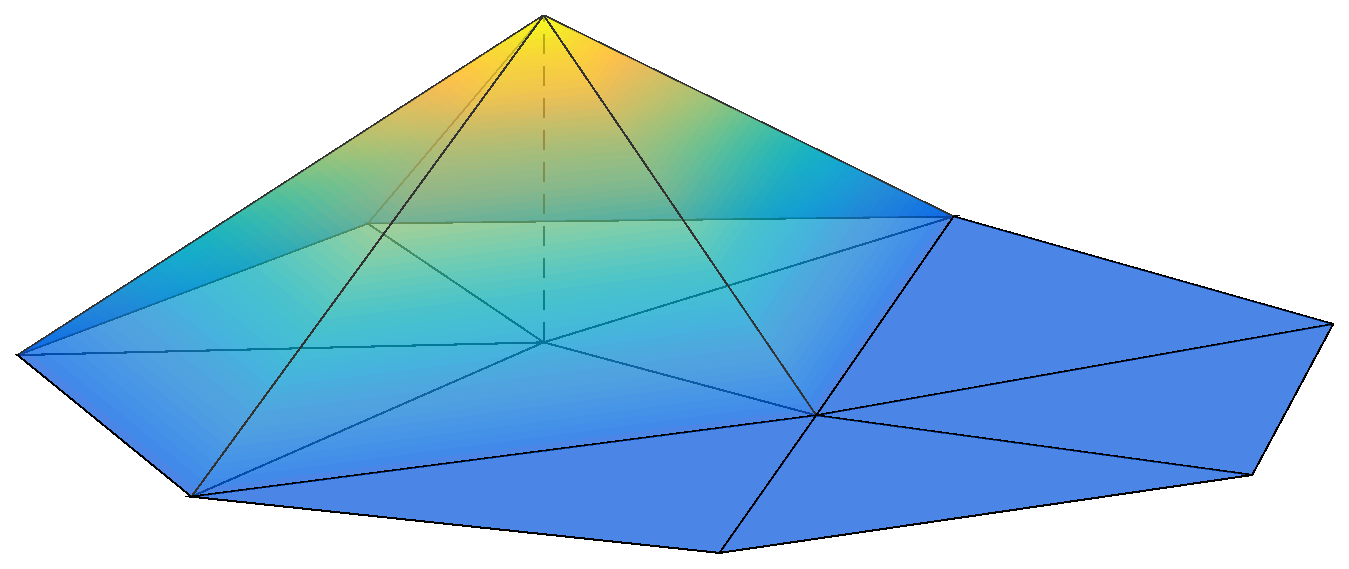
\includegraphics[width=0.48\textwidth]{shape_global_p1}
  \caption{Nodal basis $\phi_3$ for the linear finite element space $\calV_h$ defined by \eqref{eq:fe_lin_Vh}.}
  \label{fig:fe_shape_global_p1}
\end{figure}

While the choice of a basis not unique, the nodal basis provides a convenient interpretation in the physical space.  Specifically, for $w \in \calV_h$, we have a (unique) representation
\begin{equation}
  w = \sum_{j=1}^n \hat w_j \phi_j = \sum_{j=1}^n w(x_j) \phi_j.
  \label{eq:fe_rep}
\end{equation}
We note that the coefficient $\hat w_j$ must be equal to $w(x_j)$, because $w(x_i) = \sum_{j=1}^n \hat w_j \phi_j(x_i) = \sum_{j=1}^n \hat w_j \delta_{ij} = \hat w_i$, $i = 1,\dots,n$; here, the second equality follows from the Lagrange interpolation property~\eqref{eq:fe_lagrange_basis_prop}.  In words, $\hat w_j = w(x_j)$, the value of the function $w \in \calV_h$ evaluated at the associated node $x_j$. This interpretation of nodal basis allows us to readily confirm that the nodal basis is indeed a basis: for any $w \in \calV_h$, there exists a unique $\hat w \in \RR^n$ such that $w = \sum_{j=1}^n \hat w_j \phi_j$.  We can clearly express any function $w \in \calV_h$ in the form~\eqref{eq:fe_rep}; moreover the representation is unique. 

\section{Approximation spaces: essential boundary conditions}
We recall from Lecture~\ref{ch:var_form} that Dirichlet boundary conditions are treated as essential boundary conditions in the weak formulation of second-order elliptic PDEs.  For instance, given a mixed Poisson problem on $\Omega \subset \RR^d$ with a Dirichlet boundary $\Gamma_D \subset \partial \Omega$, the appropriate function space is
\begin{equation*}
  \calV \equiv \{ v \in H^1(\Omega) \ | \ v|_{\Gamma_D} = 0 \}.
\end{equation*}
The functions in the associated approximation space $\calV_h$ must also vanish on $\Gamma_D$ so that $\calV_h \subset \calV$.  With nodal basis, we can readily enforce this condition by eliminating the basis functions associated with the nodes on the (closure of the) Dirichlet boundary $\overline \Gamma_D$ from the approximation space. The dimension of the resulting approximation space for $\calV \subset H^1(\Omega)$ is
\begin{equation*}
  n = \text{dim}(\calV_h) = (\text{dimension of approximation space for $H^1(\Omega)$}) - (\text{number of Dirichlet nodes}).
\end{equation*}
Then, as before, we can express any function in $w \in \calV_h$ as
\begin{equation*}
  w = \sum_{j=1}^n \hat w_j \phi_j,
\end{equation*}
where the basis $\{ \phi_j \}_{j=1}^n$ consists of nodal basis associated with nodes not on the (closure of the) Dirichlet boundary.

We now consider the construction of an approximation space for an affine space of the form
\begin{equation*}
  \calV^E \equiv u^E + \calV,
\end{equation*}
where $u^E$ is an arbitrary member in $H^1(\Omega)$ that satisfies the boundary condition $u^E|_{\Gamma_D} = u^B$.  In general, 


\begin{equation*}
  w = u^E_h + \sum_{j=1}^n \hat w_j \phi_j
\end{equation*}
  


\section{Galerkin method}
We first recall the weak formulation for the exact problem: find $u \in \calV$ such that
\begin{equation}
  a(u,v) = \ell(v) \quad \forall v \in \calV,
  \label{eq:fe_form_true}
\end{equation}
where $a: \calV \times \calV \to \RR$ is a coercive, continuous bilinear form and $\ell: \calV \to \RR$ is a continuous linear form. We now seek an approximation to~\eqref{eq:fe_form_true} in a (finite-dimensional) subspace $\calV_h \subset \calV$: find $u_h \in \calV_h$ such that
\begin{equation}
  a(u_h,v) = \ell(v) \quad \forall v \in \calV_h.
  \label{eq:fe_form_gal_0}
\end{equation}
In words, we obtain the finite-element problem by simply replacing test and trials spaces by $\calV_h \subset \calV$.  Because the trial and test approximation spaces are the same, the method is referred to as the \emph{Galerkin method}.  (If the test and trial approximation spaces are different, the method is referred to as the \emph{Petrov-Galerkin method}.) We also note that the finite element problem~\eqref{eq:fe_form_gal_0} depends on the space $\calV_h$ but is independent of the particular basis $\{ \phi_i \}_{i=1}^n$ for $\calV_h$.  We will prove in Section~\ref{sec:fe_form_gal_wellposed} that~\eqref{eq:fe_form_gal_0} has a unique solution.

We now wish to recast the finite element problem~\eqref{eq:fe_form_gal_0} in linear algebraic from that is amenable to computer implementation.  To this end, we represent the solution and test functions in terms of their basis coefficients, $u_h = \sum_{j=1}^n \hat u_{h,j} \phi_j$ and $v = \sum_{i=1}^n \hat v \phi_i$ to yield the following equivalent problem for the coefficients: find $\hat u_h \in \RR^n$ such that
\begin{equation*}
  a(\sum_{j=1}^n \hat u_{h,j} \phi_j, \sum_{i=1}^n \hat v_i \phi_i)
  = \ell(\sum_{i=1}^n \hat v_i \phi_i) \quad \forall \hat v \in \RR^n.
\end{equation*}
We then invoke the bilinearity of $a(\cdot,\cdot)$ and the linearity of $\ell(\cdot)$ to obtain
\begin{equation*}
  \sum_{i,j = 1}^n \hat v_i a(\phi_j,\phi_i) \hat u_{h,j} = \sum_{i=1}^n \hat v_i \ell(\phi_i).
\end{equation*}
The problem can be more compactly expressed using the matrix-vector notation: find $\hat u_h \in \RR^n$ such that
\begin{equation}
  \hat v^T \hat A_h \hat u_h = \hat v^T \hat f_h \quad \forall \hat v \in \RR^n,
  \label{eq:fe_form_gal_3}
\end{equation}
where the \emph{stiffness matrix} $\hat A_h \in \RR^{n \times n}$ is given by
\begin{equation*}
  \hat A_{h,ij} \equiv a(\phi_j, \phi_i), \quad i,j = 1,\dots,n,
\end{equation*}
and the \emph{load vector} $\hat f_h \in \RR^n$ is given by
\begin{equation*}
  \hat f_{h,i} \equiv \ell(\phi_i), \quad i = 1,\dots,n.
\end{equation*}
In order for~\eqref{eq:fe_form_gal_3}, each row of $A_h \hat u_h - f_h$ must be equal to zero; otherwise, we can find $\hat v \in \RR^n$ that is finite only on that non-zero and hence~\eqref{eq:fe_form_gal_3} would not hold.  We hence conclude that the statement \eqref{eq:fe_form_gal_3} is equivalent to finding $\hat u_h \in \RR^n$ that satisfies 
\begin{equation}
  \hat A_h \hat u_h = \hat f_h  \quad \text{(in $\RR^n$)}.
  \label{eq:fe_form_gal_4}
\end{equation}
We will prove in Section~\ref{sec:fe_form_gal_wellposed} that~\eqref{eq:fe_form_gal_4} has a unique solution.

\section{Well-posedness of the Galerkin finite element formulation}
\label{sec:fe_form_gal_wellposed}
We now wish to show that~\eqref{eq:fe_form_gal_0} has a unique solution and is well-posed.
\begin{proposition}
  \label{prop:fe_form_gal_wellposed}
    Given an approximation space $\calV_h \subset \calV$, a continuous, coercive bilinear form $a: \calV \times \calV \to \RR$, and a continuous linear functional $\ell \in \calV'$, there exists a unique $u_h \in \calV_h$ such that
  \begin{equation*}
    a(u_h,v) = \ell(v) \quad \forall v \in \calV_h.
  \end{equation*}
  \begin{proof}
We will appeal to the Lax-Milgram theorem, Theorem~\ref{thm:lax_milgram}; to do so, we need to demonstrate that (i) the bilinear form $a(\cdot,\cdot)$ is coercive in $\calV_h$, (ii) the bilinear form is continuous $a(\cdot,\cdot)$ is continuous in $\calV_h$, and (iii) the linear form $\ell(\cdot)$ is continuous in $\calV_h$.  The coercivity of $a(\cdot,\cdot)$ in $\calV_h$ follows form
\begin{equation*}
  \alpha_h \equiv \inf_{v \in \calV_h} \frac{a(v,v)}{\| v \|_\calV} \geq
  \inf_{v \in \calV} \frac{a(v,v)}{\| v \|_\calV} \equiv \alpha > 0,
\end{equation*}
where the inequality follows from $\calV_h \subset \calV$.  The coercivity constant associated with $\calV_h$, $\alpha_h$, is bounded from the below by the coercivity constant associated with $\calV$, $\alpha$, which itself is bounded from the below by $0$. The continuity of $a(\cdot,\cdot)$ in $\calV_h$ follows from
\begin{equation*}
  \gamma_h \equiv \sup_{v \in \calV_h} \frac{a(v,v)}{\| v \|_\calV} \leq
  \sup_{v \in \calV} \frac{a(v,v)}{\| v \|_\calV} \equiv \gamma < \infty,
\end{equation*}
where the inequality again follows from $\calV_h \subset \calV$.  The continuity constant associated with $\calV_h$, $\gamma_h$, is bounded from the above by the continuity constant associated with $\calV$, $\gamma$, which itself is finite.  Similarly, the continuity of $\ell(\cdot)$ in $\calV_h$ follows from
\begin{equation*}
  \| \ell \|_{(\calV_h)'} \equiv \sup_{v \in \calV_h} \frac{\ell(v)}{\| v \|_\calV} \leq \sup_{v \in \calV} \frac{\ell(v)}{\| v \|_\calV} \equiv \| \ell \|_{\calV'} < \infty,
\end{equation*}
where the inequality again follows from $\calV_h \subset \calV$.  Because the bilinear from is coercive and continuous in $\calV_h$ and the linear from is continuous in $\calV_h$, we conclude by the Lax-Milgram theorem that the solution exists and is unique.
  \end{proof}
\end{proposition}
The proposition shows the existence of a unique solution to the finite element problem~\eqref{eq:fe_form_gal_0} without appealing to any specific basis for $\calV_h$; the finite element solution $u_h \in \calV_h$ (perhaps not too surprisingly) depends only on the space $\calV_h$ and is independent of the specific basis $\{ \phi_i \}_{i=1}^n$ used to represent the solution.

We can also show that the linear algebraic problem~\ref{eq:fe_form_gal_4} associated with the basis coefficients, $\hat A_h \hat u_h = \hat f_h$, is well-posed.  One way to prove the existence of unique coefficients is to appeal to (i) the existence and uniqueness of $u_h \in \calV_h$ by Proposition~\eqref{prop:fe_form_gal_wellposed} and (ii) the existence and uniqueness of the associated basis-specific representation $u_h = \sum_{i=1}^n \hat u_{h,i} \phi_i$ since $\{\phi_i\}_{i=1}^n$ is a basis for $\calV_h$. Alternatively, we can directly show that the matrix $\hat A_h \in \RR^{n \times n}$ is symmetric positive definite and hence is non-singular. 
\begin{proposition}
  If the bilinear form $a: \calV \times \calV \to \RR$ is symmetric and coercive, then the stiffness matrix $\hat A_h \in \RR^{n \times n}$ is symmetric positive definite (SPD).
  \begin{proof}
    The symmetry of $\hat A_h$ follows directly from the symmetry of the bilinear form:
  \begin{equation*}
    \hat A_{h,ij} = a(\phi_j,\phi_i) = a(\phi_i,\phi_j) = \hat A_{h,ji}.
  \end{equation*}
  To prove positive definiteness, we first observe that $\forall \hat v \in \RR^n$, 
\begin{equation*}
  \hat v^T \hat A_{h} \hat v
  =
  \sum_{i,j = 1}^n \hat v_i a(\phi_j, \phi_i) \hat v_j 
  = a(\sum_{j=1}^n \hat v_j \phi_j, \sum_{i=1}^n \hat v_i \phi_i)
  \geq \alpha \| \sum_{i=1}^n \hat v_i \phi_i \|^2_{\calV} \geq 0,
\end{equation*}
where the first inequality follows from the coercivity of $a(\cdot,\cdot)$ and the last equality follows from the positive definiteness of the norm $\| \cdot \|_{\calV}$. Moreover, because $\| \cdot \|_{\calV}$ is a norm, $\| \sum_{i=1}^n \hat v_i \phi_i \|_\calV = 0$ if and only if $\sum_{i=1}^n \hat v_i \phi_i = 0$.  In addition, because $\{\phi_i\}_{i=1}^n$ is a basis and in particular linearly independent, $\sum_{i=1}^n \hat v_i \phi_i = 0$ if and only if $\hat v_i = 0$, $\forall i = 1,\dots,n$. It follows that
\begin{equation*}
  \hat v^T \hat A_h \hat v = 0 \quad \text{if and only if} \quad \hat v = 0.
\end{equation*}
Hence, the matrix $\hat A_h \in \RR^{n \times n}$ is SPD.
  \end{proof}
\end{proposition}


\section{Minimization formulation: Rayleigh-Ritz formulation}
We now seek the finite element approximation to the problem using the minimization formulation. To this end, we recall that the energy functional is given by 
\begin{align*}
  J(w) =  J(\sum_{j=1}^n \hat w_j \phi_j)
  = \frac{1}{2} a (\sum_{j=1}^n \hat w_j \phi_j, \sum_{i=1}^n \hat w_i \phi_i) - \ell(\sum_{i=1}^n \hat w_i \phi_i)
  = \frac{1}{2} \sum_{i,j=1}^n \hat w_i a(\phi_j,\phi_i) \hat w_j - \sum_{i=1}^n \hat w_i \ell(\phi_i)
\end{align*}

\begin{equation*}
  (\hat A_h)_{ij} \equiv a(\phi_j,\phi_i)
  \quad \text{and} \quad
  (\hat f_h)_i \equiv \ell(\phi_i)
\end{equation*}

\begin{equation*}
  \hat J(\hat w) = J(\sum_{j=1}^n \hat w_j \phi_j)
  = \frac{1}{2} \hat w^T \hat A_h \hat w - \hat w^T \hat f_h
\end{equation*}

\begin{equation*}
  \hat u_h = \argmin_{\hat w \in \RR^n} \hat J(\hat w)
\end{equation*}

\begin{equation*}
  \nabla \hat J(\hat u_h) = \hat A_h \hat u_h - \hat f_h = 0
\end{equation*}

\section{Generalization}
In this lecture, we considered an approximation space based on piecewise polynomials and constructed the associated Galerkin (and Rayleigh-Ritz) approximation. However, the Galerkin (and Rayleigh-Ritz) procedure are in fact general projection procedure that works with any approximation spaces. For instance, the \emph{spectral method} is an approximation 
\begin{equation*}
  \calV_p \equiv \{ v \in \calV \ | \ v \in \PP^p(\Omega) \}.
\end{equation*}
